En el presente capítulo se expone el análisis realizado en base a los requisitos
presentados en el capítulo~\ref{chap:requisitos}, haciendo uso del lenguaje de
modelado UML. Se describen:

\begin{itemize}
\item El \textbf{modelo conceptual} de los datos usados en la aplicación,
  elaborado a partir de los requisitos de información.
\item Los \textbf{casos de uso}, que describen los pasos que componen los
  procesos habituales del proyecto.
\item El \textbf{modelo de interfaz de usuario}, en el que se presenta un
  prototipo de la navegación y de las interfaces de la aplicación móvil.
\end{itemize}

\section{Modelo conceptual}

En base a los requisitos especificados en la
sección~\ref{sec:requisitos-informacion} el modelo conceptual es el que se
refleja en la imagen~\ref{fig:modelo-conceptual}. En él que se identifican los
principales tipos de datos, con sus atributos y relaciones.

A continuación se detallan cada uno de los tipos de datos reflejados en el
modelo conceptual.


\subsection{Usuario}

Representa a un usuario de la aplicación que puede crear y modificar recetas,
además de añadir comentarios y valorarlas.

\begin{description}
\item[Nombre de usuario] Identificador único del usuario.
\item[Contraseña] Contraseña para el login del usuario.
\item[Correo electrónico] Dirección de correo electrónico.
\item[Nombre] Nombre del usuario.
\item[Apellidos] Apellidos del usuario.
\item[Fecha de cumpleaños] Día del cumpleaños del usuario.
\end{description}

\textbf{Relaciones}
\begin{itemize}
\item Un \textbf{usuario} puede crear \textbf{recetas}.
\item Un \textbf{usuario} puede comentar recetas (o crear
\textbf{comentarios de recetas}).
\item Un \textbf{usuario} puede valorar recetas (o crear
\textbf{puntuaciones de recetas}).
\end{itemize}


\begin{figure}[H]
  \centering
  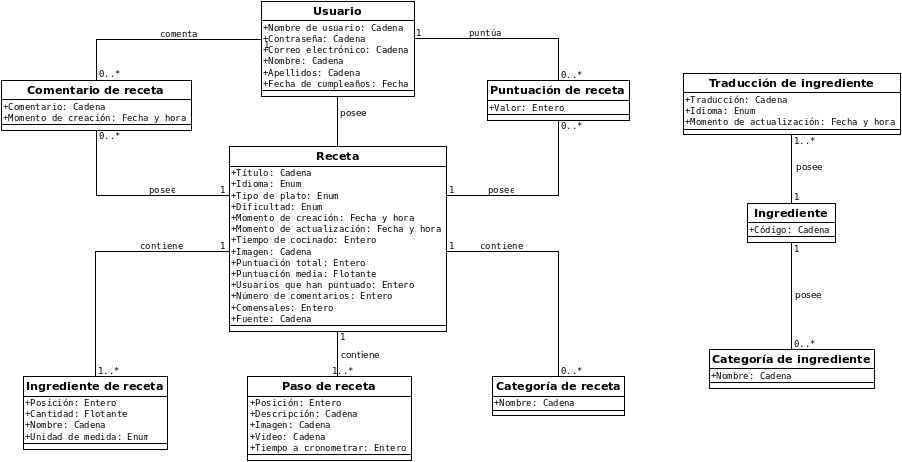
\includegraphics[width=\textwidth]{cap4/img/diagrama_clases_conceptuales}
  \caption{Modelo conceptual}
  \label{fig:modelo-conceptual}
\end{figure}

\subsection{Receta}

Representa a una receta de cocina.

\begin{description}
\item[Título] Nombre identificativo de la receta.
\item[Idioma] Idioma en el que está escrita la receta.
\item[Tipo de plato] Tipo de plato de la receta (entrante, primero,...).
\item[Dificultad] Dificultad que implica hacer la receta (baja, media, alta).
\item[Momento de creación] Instante en el que se creó la receta.
\item[Momento de actualización] Instante en el que se actualizó por última vez
la receta.
\item[Tiempo de cocinado] Tiempo que se tarda en ejecutar por completo la receta.
\item[Imagen] URL de la imagen asociada a la receta.
\item[Puntuación total] Contador total de la puntuación de todos los usuarios que
han valorado la receta.
\item[Usuarios que han puntuado] Contador total de la cantidad de usuarios que
han valorado la receta.
\item[Puntuación media] Media de valoración de la receta (puntuación total
dividida entre número de usuarios).
\item[Número de comentarios] Cantidad de comentarios que han hecho los usuarios
en la receta.
\item[Comensales] Cantidad de personas que pueden ser servidas con esta receta.
\item[Fuente] Origen del cual se obtuvo la receta (normalmente, una URL).
\end{description}

\textbf{Relaciones}
\begin{itemize}
\item Una \textbf{receta} pertenece a un \textbf{usuario}.
\item Una \textbf{receta} posee una lista de \textbf{ingredientes de receta}.
\item Una \textbf{receta} posee una lista de \textbf{pasos de receta}.
\item Una \textbf{receta} posee una lista de \textbf{categorías de receta}.
\end{itemize}


\subsection{Ingrediente de receta}

Representa a un ingrediente de una receta.

\begin{description}
\item[Posición] Posición del ingrediente en el listado de ingredientes.
\item[Nombre] Nombre identificativo del ingrediente.
\item[Cantidad] Cantidad del ingrediente a usar en la receta.
\item[Unidad de medida] Unidad en que se mide la cantidad del ingrediente.
\end{description}


\textbf{Relaciones}
\begin{itemize}
\item Un \textbf{ingrediente de receta} pertenece a una \textbf{receta}.
\end{itemize}


\subsection{Paso de receta}

Representa a un paso de una receta.

\begin{description}
\item[Posición] Posición del ingrediente en el listado de ingredientes.
\item[Descripción] Descripción de lo que hay que hacer en el paso de la receta.
\item[Imagen] URL de la imagen asociada al paso.
\item[Video] URL del video asociada al paso.
\item[Tiempo a cronometrar] Tiempo de espera tras la realización del paso.
\end{description}


\textbf{Relaciones}
\begin{itemize}
\item Un \textbf{paso de receta} pertenece a una \textbf{receta}.
\end{itemize}


\subsection{Categoría de receta}

Representa a una categoría de una receta, que indica a qué dieta pertenece la
receta o si contiene ingredientes que sean alérgenos.

\begin{description}
\item[Nombre] Nombre indentificativo de la categoría.
\end{description}


\textbf{Relaciones}
\begin{itemize}
\item Una \textbf{categoría de receta} pertenece a una \textbf{receta}.
\end{itemize}


\subsection{Comentario de receta}

Representa a un comentario de una receta realizado por un usuario.

\begin{description}
\item[Comentario] Contenido del comentario.
\item[Momento de creación] Instante en el que se creó el comentario.
\end{description}


\textbf{Relaciones}
\begin{itemize}
\item Un \textbf{comentario de receta} pertenece a una \textbf{receta}.
\item Un \textbf{comentario de receta} es creado por un \textbf{usuario}.
\end{itemize}


\subsection{Puntuación de receta}

Representa a una puntuación de una receta valorada por un usuario.

\begin{description}
\item[Comentario] Contenido del comentario.
\item[Momento de creación] Instante en el que se creó el comentario.
\end{description}


\textbf{Relaciones}
\begin{itemize}
\item Una \textbf{puntuación de receta} pertenece a una \textbf{receta}.
\item Una \textbf{puntuación de receta} es valorada por un \textbf{usuario}.
\end{itemize}


\subsection{Ingrediente}

Representa a un ingrediente que puede ser válido introducir en una receta.

\begin{description}
\item[Código] Nombre identificativo del ingrediente.
\end{description}


\textbf{Relaciones}
\begin{itemize}
\item Un \textbf{ingrediente} posee una o varias \textbf{categorías de
ingrediente}.
\item Un \textbf{ingrediente} posee una o varias \textbf{traducciones de
ingrediente}.
\end{itemize}


\subsection{Categoría de ingrediente}

Representa a una categoría de un ingrediente, que indica si es ingrediente
es un alérgeno.

\begin{description}
\item[Nombre] Nombre identificativo de la categoría.
\end{description}


\textbf{Relaciones}
\begin{itemize}
\item Una \textbf{categoría de ingrediente} pertenece a un \textbf{ingrediente}.
\end{itemize}


\subsection{Traducción de ingrediente}

Representa a una traducción de un ingrediente para un idioma.

\begin{description}
\item[Traducción] Traducción del ingrediente.
\item[Idioma] Idioma en el que está traducido.
\item[Momento de actualización] Instante en el que se actualizó por última vez
la receta.
\end{description}


\textbf{Relaciones}
\begin{itemize}
\item Una \textbf{categoría de ingrediente} pertenece a un \textbf{ingrediente}.
\end{itemize}




\section{Modelo de casos de uso}

El modelo de casos de uso representa las interacciones entre los actores y el
sistema, desarrollado a partir de los requisitos descritos anteriormente.

\subsection{Actores}


En este apartado se describen los diversos roles que pueden poseer los usuarios
del sistema, según se visualiza en la imagen \ref{fig:actores}.

\begin{figure}[h]
  \centering
  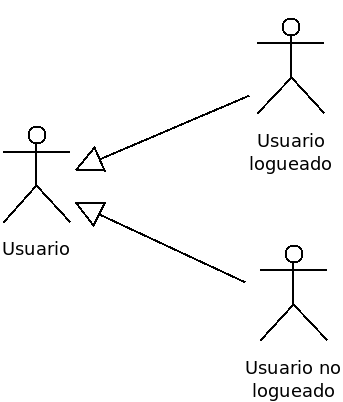
\includegraphics[width=0.4\textwidth]{cap4/img/diagrama_actores}
  \caption{Diagrama de actores}
  \label{fig:actores}
\end{figure}


\subsubsection{Usuario}

\begin{center}
  \begin{tabularx}{\textwidth}{|c|X|}
    \hline
     & Usuario \\

    \hline

    Descripción & Usuario de la aplicación, que puede haber hecho login
    previamente o no. \\

    \hline
  \end{tabularx}

\end{center}


\subsubsection{Usuario logueado}

\begin{center}
  \centering
  \begin{tabularx}{\textwidth}{|c|X|}
    \hline
     & Usuario logueado \\

    \hline

    Descripción & Usuario que, estando ya registrado, se ha logueado en el
    sistema. \\

    \hline
  \end{tabularx}
\end{center}


\subsection{Subsistema de gestión de usuarios}

Los casos de uso pertenecientes a este subsistema pueden verse en la
figura~\ref{fig:subsistema-usuarios}

\begin{figure}[hp]
  \centering
  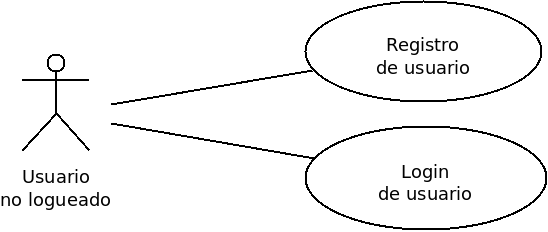
\includegraphics[width=0.5\textwidth]{cap4/img/diagrama_subsistema_usuarios}
  \caption{Casos de uso del subsistema de gestión de usuarios}
  \label{fig:subsistema-usuarios}
\end{figure}

\subsubsection{Caso de uso: acceso a la aplicación}

\begin{description}
\item[Descripción] Un usuario logueado o no accede a la aplicación.
\item[Actores] \textit{Usuario}.
\item[Escenario principal] $\quad$
  \begin{enumerate}
  \item Un usuario decide acceder a la aplicación y pulsa sobre el icono.
  \item El \textit{sistema} comprueba si hay nuevos ingredientes por descargar
  y descarga los ingredientes necesarios y los almacena en el sistema.
  \item El \textit{sistema} comprueba si el usuario ha guardado sus credenciales
  y loguea al usuario.
  \item El \textit{sistema} continua hasta la pantalla principal y descarga
  \end{enumerate}
\item[Flujo alternativo] $\quad$
  \begin{description}
  \item[2a] No hay conexión a internet. El sistema continua por el paso 3.
  \item[3a] No hay conexión a internet. El sistema continua por el paso 4.
  \end{description}
\end{description}


\subsubsection{Caso de uso: registro de usuario}

\begin{description}
\item[Descripción] Un usuario no logueado se registra en la aplicación para
poder subir las recetas.
\item[Actores] \textit{Usuario no logueado}.
\item[Escenario principal] $\quad$
  \begin{enumerate}
  \item Un usuario decide registrarse en el sistema y accede a la vista de
  registro.
  \item El \textit{usuario} introduce su dirección de correo electrónico y
  contraseña, además de su nombre y apellidos.
  \item El \textit{sistema} comprueba que los datos introducidos son correctos.
  \item El \textit{sistema} registra al usuario.
  \end{enumerate}
\item[Flujo alternativo] $\quad$
  \begin{description}
  \item[3a] Alguno de los datos introducidos es incompleto o no es correcto. El
    sistema informa al usuario del error.
  \item[3b] La dirección de correo electrónico ya han sido usados previamente.
  El sistema informa al usuario del error.
  \end{description}
\end{description}


\subsubsection{Caso de uso: login de usuario}

\begin{description}
\item[Descripción] Un usuario no logueado previamente registrado quiere loguearse
en la aplicación.
\item[Actores] \textit{Usuario no logueado}.
\item[Escenario principal] $\quad$
  \begin{enumerate}
  \item Un usuario decide hacer login en el sistema y accede a la vista de login.
  \item El \textit{usuario} introduce su nombre de usuario y contraseña.
  \item El \textit{sistema} comprueba que los datos introducidos son correctos.
  \item El \textit{sistema} loguea al usuario.
  \end{enumerate}
\item[Flujo alternativo] $\quad$
  \begin{description}
  \item[3a] Alguno de los datos introducidos no tiene el formato correcto o está
    en blanco. El sistema informa al usuario del error.
  \item[3b] Los datos introducidos no corresponden a ningún usuario registrado.
  El sistema informa al usuario del error.
  \end{description}
\end{description}



\subsection{Subsistema de gestión de recetas}

Los casos de uso pertenecientes a este subsistema pueden verse en la
figura~\ref{fig:subsistema-recetas}

\begin{figure}[hp]
  \centering
  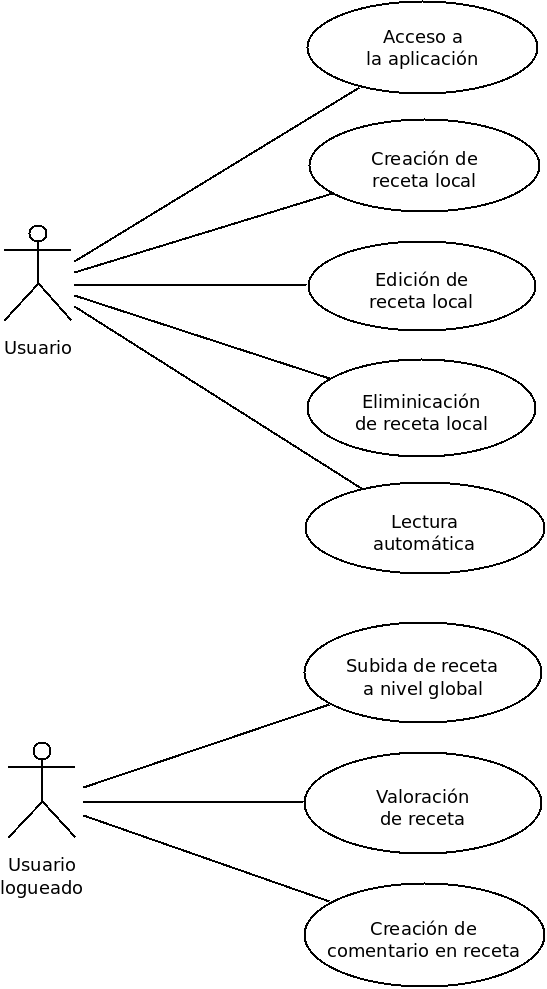
\includegraphics[width=0.5\textwidth]{cap4/img/diagrama_subsistema_recetas}
  \caption{Casos de uso del subsistema de gestión de recetas}
  \label{fig:subsistema-recetas}
\end{figure}

\subsubsection{Caso de uso: creación de receta local}

\begin{description}
\item[Descripción] Un usuario logueado o no logueado crea una receta a nivel
local.
\item[Actores] \textit{Usuario}.
\item[Escenario principal] $\quad$
  \begin{enumerate}
  \item El usuario decide crear una nueva receta y accede a la vista principal.
  \item El usuario pulsa sobre el botón de \textit{Añadir receta}.
  \item El \textit{usuario} introduce su dirección de correo electrónico y
  contraseña, además de su nombre y apellidos.
  \item El sistema accede a la vista para añadir una nueva receta.
  \item El usuario introduce el título, el tipo de plato, la dificultad, el
  tiempo de cocinado, la imagen (si lo desea), el número de comensales y la
  fuente, además del listado de ingredientes y pasos y las categorías necesarias.
  \item El \textit{sistema} comprueba que los datos introducidos son correctos.
  \item El \textit{sistema} revisa todos los ingredientes y modifica las
  categorías de la receta conforme a estos si fuera necesario.
  \item El \textit{sistema} guarda la receta.
  \end{enumerate}
\item[Flujo alternativo] $\quad$
  \begin{description}
  \item[6a] Alguno de los datos introducidos es incompleto o no es correcto. El
    sistema informa al usuario del error.
  \end{description}
\end{description}


\subsubsection{Caso de uso: edición de receta local}

\begin{description}
\item[Descripción] Un usuario logueado o no logueado actualiza una receta a nivel
local.
\item[Actores] \textit{Usuario}.
\item[Escenario principal] $\quad$
  \begin{enumerate}
  \item El \textit{usuario} decide editar una receta ya existente y accede a la
  vista principal.
  \item El \textit{usuario} busca la receta a editar y pulsa sobre ella para
  acceder a su detalle.
  \item El \textit{usuario} pulsa sobre el botón \textit{Editar receta} para
  acceder a la vista de edición.
  \item El \textit{usuario} modifica cualquiera de los datos de la receta.
  \item El \textit{sistema} comprueba que los datos introducidos son correctos.
  \item El \textit{sistema} revisa todos los ingredientes y modifica las
  categorías de la receta conforme a estos si fuera necesario.
  \item El \textit{sistema} actualiza la receta.
  \end{enumerate}
\item[Flujo alternativo] $\quad$
  \begin{description}
  \item[5a] Alguno de los datos introducidos es incompleto o no es correcto. El
    sistema informa al usuario del error.
  \end{description}
\end{description}


\subsubsection{Caso de uso: eliminación de receta local}

\begin{description}
\item[Descripción] Un usuario logueado o no logueado borra una receta a nivel
local.
\item[Actores] \textit{Usuario}.
\item[Escenario principal] $\quad$
  \begin{enumerate}
  \item El \textit{usuario} decide borrar una receta ya existente y accede a la
  vista principal.
  \item El \textit{usuario} busca la receta a editar y pulsa sobre ella para
  acceder a su detalle.
  \item El \textit{usuario} pulsa sobre el botón \textit{Eliminar receta}.
  \item El \textit{sistema} muestra un mensaje para confirmar la eliminación.
  \item El \textit{usuario} confirma la eliminación.
  \item El \textit{sistema} elimina la receta.
  \end{enumerate}
\item[Flujo alternativo] $\quad$
  \begin{description}
  \item[4a] El \textit{usuario} no confirma la eliminación. El \textit{sistema}
  oculta el mensaje de confirmación.
  \end{description}
\end{description}



\subsubsection{Caso de uso: subida de receta a nivel global}

\begin{description}
\item[Descripción] Un usuario logueado comparte una receta ya existente a nivel
global.
\item[Actores] \textit{Usuario logueado}.
\item[Escenario principal] $\quad$
  \begin{enumerate}
  \item El \textit{usuario} decide compartir una receta ya existente y accede a
  la vista principal.
  \item El \textit{usuario} busca la receta a editar y pulsa sobre ella para
  acceder a su detalle.
  \item El \textit{usuario} pulsa sobre el botón \textit{Subir receta}.
  \item El \textit{sistema} envía la petición para crear la receta a nivel
  global.
  \end{enumerate}
\end{description}


\subsubsection{Caso de uso: valoración de receta}

\begin{description}
\item[Descripción] Un usuario logueado valora una receta ya existente a nivel
global.
\item[Actores] \textit{Usuario logueado}.
\item[Escenario principal] $\quad$
  \begin{enumerate}
  \item El \textit{usuario} decide valorar una receta ya existente y accede a
  la vista principal.
  \item El \textit{usuario} busca la receta a valorar y pulsa sobre ella para
  acceder a su detalle.
  \item El \textit{usuario} pulsa sobre el botón \textit{Valorar receta}.
  \item El \textit{sistema} pregunta qué puntuación se desea dar a la receta.
  \item El \textit{usuario} introduce su puntuación.
  \item El \textit{sistema} guarda la valoración de la receta.
  \end{enumerate}
\item[Flujo alternativo] $\quad$
  \begin{description}
  \item[5a] El \textit{usuario} no introduce su puntuación. El \textit{sistema}
  oculta la pregunta de la puntuación.
  \end{description}
\end{description}


\subsubsection{Caso de uso: creación de comentario en receta}

\begin{description}
\item[Descripción] Un usuario logueado comenta una receta ya existente a nivel
global.
\item[Actores] \textit{Usuario logueado}.
\item[Escenario principal] $\quad$
  \begin{enumerate}
  \item El \textit{usuario} decide comentar una receta ya existente y accede a
  la vista principal.
  \item El \textit{usuario} busca la receta a comentar y pulsa sobre ella para
  acceder a su detalle.
  \item El \textit{usuario} introduce el mensaje y pulsa sobre el botón
  \textit{Enviar comentario}.
  \item El \textit{sistema} envía el comentario.
  \end{enumerate}
\end{description}



\subsubsection{Caso de uso: lectura automática}

\begin{description}
\item[Descripción] Un usuario logueado o no logueado quiere que el sistema lea
automáticamente la receta.
\item[Actores] \textit{Usuario}.
\item[Escenario principal] $\quad$
  \begin{enumerate}
  \item El \textit{usuario} decide que el sistema le lea la receta y accede a
  la vista principal.
  \item El \textit{usuario} busca la receta y pulsa sobre ella para acceder a su
  detalle.
  \item El \textit{usuario} pulsa el botón de \textit{Lectura automática}.
  \item El \textit{sistema} identifica el primer paso como el siguiente.
  \item El \textit{sistema} lee el paso siguiente.
  \item El \textit{sistema} pregunta cuál es la siguiente opción a ejecutar:
  \begin{enumerate}
  \item Leer el paso siguiente.
  \item Volver a leer el paso actual.
  \item Cronometrar el tiempo de espera.
  \item Salir de la lectura automática.
  \end{enumerate}
  \item El \textit{usuario} escoge la opción de salir.
  \item El \textit{sistema} finaliza la ejecución.
  \end{enumerate}
\item[Flujo alternativo] $\quad$
  \begin{description}
  \item[7a] El \textit{usuario} escoge la opción de leer el paso siguiente. El
  \textit{sistema} identifica el siguiente paso después del actual y se vuelve
  a ejecutar el flujo desde el paso 5.
  \item[7b] El \textit{usuario} escoge la opción de volver a leer el paso actual.
  Se vuelve a ejecutar el flujo desde el paso 5.
  \item[7c] El \textit{usuario} escoge la opción de cronometrar el tiempo de
  espera. El \textit{sistema} inicia el temporizador. Al finalizar, se vuelve a
  ejecutar el flujo desde el paso 6.
  \item[7c-2] El \textit{usuario} cancela el temporizador. Se vuelve a ejecutar
  el flujo desde el paso 6.
  \item[7d] El \textit{usuario} no introduce ninguna opción reconocible por el
  \textit{sistema}. Se vuelve a ejecutar el flujo desde el paso 6.
  \end{description}

\end{description}



\section{Modelo de interfaz de usuario}

\subsection{Modelo de navegación}

El modelo de navegación de la aplicación móvil se presenta en la
figura~\ref{fig:modelo-navegacion}.

\begin{figure}[hp]
  \centering
  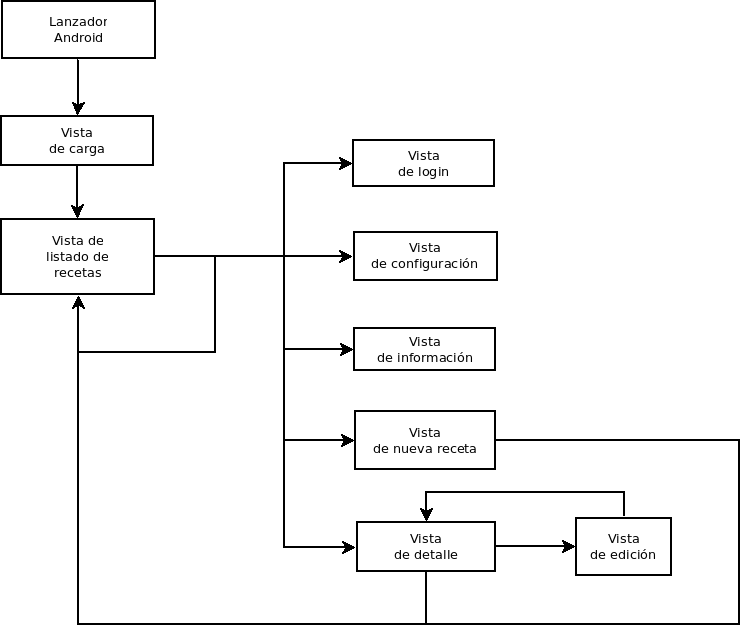
\includegraphics[width=\textwidth]{cap4/img/diagrama_navegacion}
  \caption{Modelo de navegación}
  \label{fig:modelo-navegacion}
\end{figure}


\subsection{Prototipos visuales}

A continuación se presentan los prototipos de las interfaces visuales de la
aplicación móvil.

\begin{itemize}
\item La figura~\ref{fig:diagrama-prototipo-carga} representa la vista de carga
de la aplicación Android.
\item La figura~\ref{fig:diagrama-prototipo-vista-principal} representa la vista
del listado de recetas.
\item La figura~\ref{fig:diagrama-prototipo-menu} representa la vista
del menú lateral que da acceso a las demás vistas.
\item La figura~\ref{fig:diagrama-prototipo-filtrado} representa la vista
del filtrado de recetas que aparece desde el otro lateral.
\item La figura~\ref{fig:diagrama-prototipo-login} representa la vista
de login.
\item La figura~\ref{fig:diagrama-prototipo-registro} representa la vista
de registro.
\item La figura~\ref{fig:diagrama-prototipo-detalle} representa la vista
de detalle de una receta.
\item Las figuras~\ref{fig:diagrama-prototipo-edicion},
\ref{fig:diagrama-prototipo-edicion-ingredientes} y
~\ref{fig:diagrama-prototipo-edicion-nuevo-ingrediente} representan la vista
de edición de una receta, junto con la edición de elementos particulares, como
los ingredientes (análogo para los pasos).
\item La figura~\ref{fig:diagrama-prototipo-config} representa la vista
de configuración de la aplicación móvil.
\end{itemize}

\begin{figure}[hp]
  \centering
  \includegraphics[width=0.3\textwidth]{cap4/img/diagrama_prototipo_carga}
  \caption{Vista de carga}
  \label{fig:diagrama-prototipo-carga}
\end{figure}

\begin{figure}[hp]
  \centering
  \includegraphics[width=0.7\textwidth]{cap4/img/diagrama_prototipo_vista_principal}
  \caption{Vista de listado de recetas}
  \label{fig:diagrama-prototipo-vista-principal}
\end{figure}

\begin{figure}[hp]
  \centering
  \includegraphics[width=0.5\textwidth]{cap4/img/diagrama_prototipo_menu}
  \caption{Vista de menú}
  \label{fig:diagrama-prototipo-menu}
\end{figure}

\begin{figure}[hp]
  \centering
  \includegraphics[width=0.5\textwidth]{cap4/img/diagrama_prototipo_filtrado}
  \caption{Vista de filtrado}
  \label{fig:diagrama-prototipo-filtrado}
\end{figure}

\begin{figure}[hp]
  \centering
  \includegraphics[width=0.3\textwidth]{cap4/img/diagrama_prototipo_login}
  \caption{Vista de login}
  \label{fig:diagrama-prototipo-login}
\end{figure}

\begin{figure}[hp]
  \centering
  \includegraphics[width=0.3\textwidth]{cap4/img/diagrama_prototipo_registro}
  \caption{Vista de registro}
  \label{fig:diagrama-prototipo-registro}
\end{figure}

\begin{figure}[hp]
  \centering
  \includegraphics[width=0.7\textwidth]{cap4/img/diagrama_prototipo_detalle}
  \caption{Vista de detalle}
  \label{fig:diagrama-prototipo-detalle}
\end{figure}

\begin{figure}[hp]
  \centering
  \includegraphics[width=0.7\textwidth]{cap4/img/diagrama_prototipo_edicion}
  \caption{Vista de edición y creación}
  \label{fig:diagrama-prototipo-edicion}
\end{figure}

\begin{figure}[hp]
  \centering
  \includegraphics[width=0.7\textwidth]{cap4/img/diagrama_prototipo_edicion_ingredientes}
  \caption{Vista de edición y creación - Ingredientes}
  \label{fig:diagrama-prototipo-edicion-ingredientes}
\end{figure}

\begin{figure}[hp]
  \centering
  \includegraphics[width=0.7\textwidth]{cap4/img/diagrama_prototipo_edicion_nuevo_ingrediente}
  \caption{Vista de edición y creación - Nuevo ingrediente}
  \label{fig:diagrama-prototipo-edicion-nuevo-ingrediente}
\end{figure}

\begin{figure}[hp]
  \centering
  \includegraphics[width=0.5\textwidth]{cap4/img/diagrama_prototipo_config}
  \caption{Vista de configuración}
  \label{fig:diagrama-prototipo-config}
\end{figure}
